\documentclass{article}
\usepackage[english]{babel}
\usepackage[a4paper,top=2.54cm,bottom=2.54cm,left=2.54cm,right=2.54cm,marginparwidth=1.75cm]{geometry}
\usepackage{amsmath}
\usepackage{graphicx}
\usepackage{amsfonts}
\usepackage{amssymb}
\usepackage{enumerate}
\usepackage{enumitem}
\usepackage[colorlinks=true, allcolors=blue]{hyperref}
\usepackage{graphicx}
\usepackage[export]{adjustbox}
\usepackage{multirow}
\usepackage{MnSymbol}%
\usepackage{wasysym}%
\title{Calculus A(1): Homework 8}
\begin{document}
\maketitle
\section*{4.4.}
\subsection*{80.}
\textbf{Horizontal tangents   }True, or false? Explain.
\begin{enumerate} [label=\textbf{\alph*.}]
    \item The graph of every polynomial of even degree (largest exponent even) has at least one horizontal tangent.
    \item  The graph of every polynomial of odd degree (largest exponent odd) has at least one horizontal tangent.
\end{enumerate}

\subsection*{Solution.}
\begin{enumerate} [label=\textbf{\alph*.}]
    \item \textbf{True}.\newline
    Let $f(x)$ be the polynomial.\newline
    (1). It is clear that the degree of the derivative of a polynomial would have a decrement of 1 w.r.t. the polynomial itself, so $f'(x)$ is a polynomial with odd degree.\newline
    $f'(x)$ is odd-degree-polynomial, so by intermediate value theorem, $f'(x)$ must have at least one real root.\newline
    (2). Since any point that its tangent is a horizontal line must be an extremum,  the point must have the derivative of the polynomial zero. \newline
    (1) and (2) together which proved the existence of a horizontal tangent.
    \item \textbf{False}. $f(x)=x$ is a polynomial of odd degree, however $f'(x)=1$ is never a horizontal tangent.
\end{enumerate}
\subsection*{84.}
\textbf{Cubic curves } What can you say about the inflection points of a cubic curve $y=ax^3+bx^2+cx+d,a\neq 0$? Give reasons for your answer.
\subsection*{Solution.}
$(x_0,y|_{x=x_0})$ is a inflection point if $x_0$ satisfies $y''=0$.
\[y''=6ax+2b\]
So
\[x_0=-\frac{b}{3a}\]
This point exists and is unique. As $y''$ is shown to be continuous in $\mathbf{R}$, and is linear, $x_0=-b/(3a)$ is the only inflection point of $y$.
\subsection*{91.}
\begin{enumerate}[label=\textbf{\alph*.}]
    \item On a common screen, graph $f(x)=x^3+kx$ for $k=0$ and nearby positive and negative values of k. How does the value of $k$ seem to affect the shape of the graph?
    \item Find $f'(x)$. As you will see, $f'(x)$ is a quadratic function of x. Find the discriminant of the quadratic (the discriminant of $ax^2+bx+c$ is $b^2-4ac$). For what values of $k$ is the discriminant positive? Zero? Negative? For what values of $k$ does $f'$ have two zeros? One or no zeros? Now explain what the value of $k$ has to do with the shape of the graph of $f$.
    \item Experiment with other values of $k$. What appears to happen as $k\to-\infty$? as $k\to \infty$?
\end{enumerate}
\subsection*{Solution.}
\begin{enumerate}[label=\textbf{\alph*.}]
    \item \text{   }\newline
    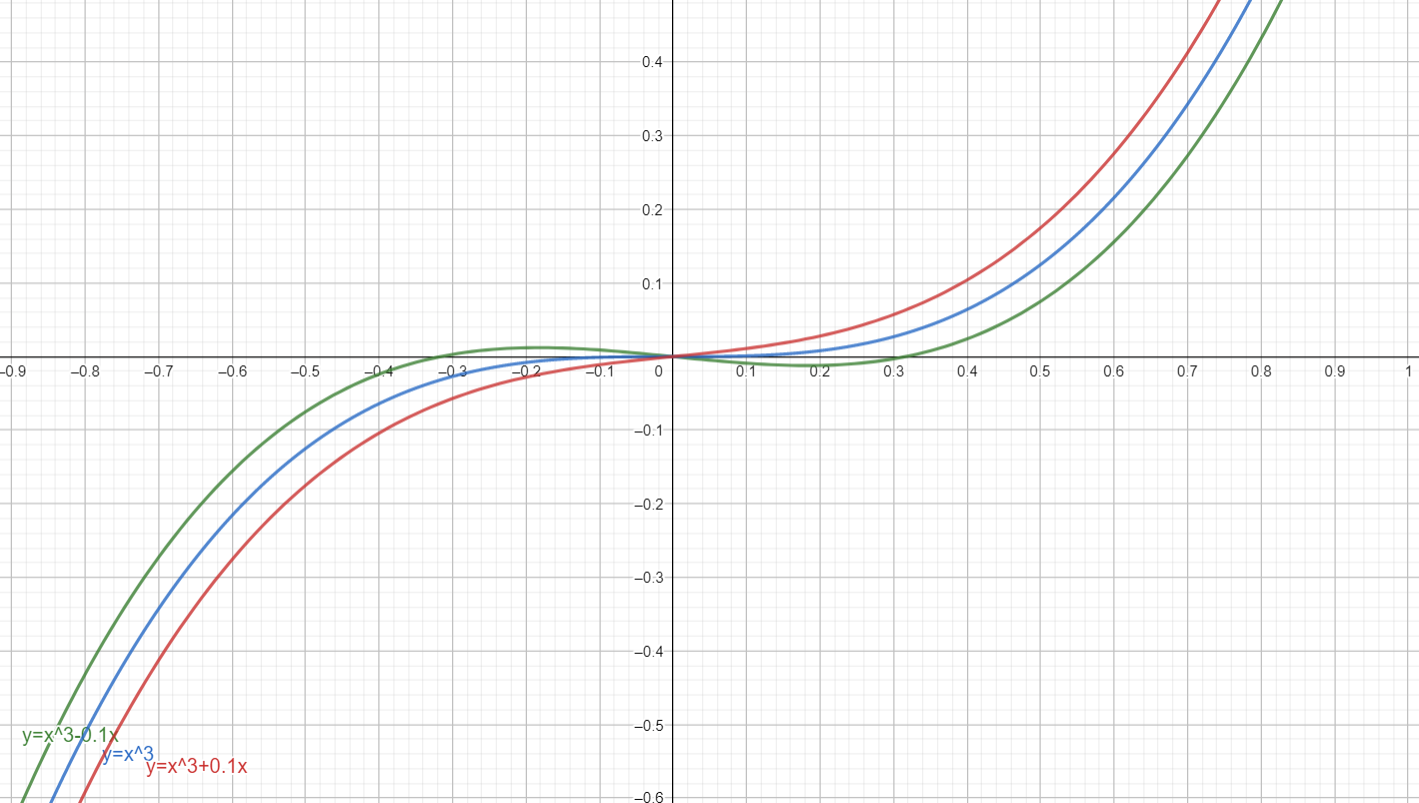
\includegraphics[scale=0.25]{img/圖片_2021-12-12_002741.png}\newline
    As seen by the graphs of the three functions, it seems that $k$ manipulates the existence and the magnitude of the extrema of the polynomial.\newline
    For negative values of $k$, it appears that magnitude of the extrema increases with the magnitude of $k$.
    For positive value of $k$, the graph appears to be steep, which has positive slope everywhere.
    \item \[f'(x)=3x^2+k\]
    \[\Delta=-4*3*k=-12k\]
    Let $x_0$ satisfies $f'(x_0)=0$.
    Then
    \[x_0=\pm\sqrt{-\frac{k}{3}}\]
    \[f' \text{  have two zeros  }\Leftrightarrow \Delta>0\Leftrightarrow k<0\]
    \[f' \text{  have one zero  }\Leftrightarrow \Delta=0\Leftrightarrow k=0\]
    \[f' \text{  have no zeros  }\Leftrightarrow \Delta<0\Leftrightarrow k>0\]
    \item By continuing the manipulation of $k$ from (a), when $k\to+\infty$, the locus of points of the graph seems to satisfy $x=0$.\newline
    When $k\to -\infty$, the two extrema tend to behave like points at infinity on the second and forth quadrants.
\end{enumerate}
\section*{4.6.}
\subsection*{33.}
\textbf{Continuous extension}   Find a value of $c$ that makes the function
\[f(x)=\left\{\begin{array}{ll}
\frac{9x-3\sin{3x}}{5x^3}, & x\neq 0 \\
c & x=0
\end{array}\right.\]
continuous at $x=0$. Explain why your value of $c$ works.
\subsection*{Solution.}
$f$ is continuous at $x=0$ 
\[\Leftrightarrow \lim _{x\to 0} f(x)=f(0)=c\]
\[\Leftrightarrow c=\lim _{x\to 0} \frac{9x-3 \sin 3x}{5x^3}=\lim _{x\to 0} \frac{9-9 \cos 3x}{15x^2}=\lim _{x\to 0} \frac{27 \sin 3x}{30x}=\lim _{x\to 0} \frac{81 \cos 3x}{30}=\frac{81}{30}=2.7\]
\subsection*{39.}
In the accompanying figure, \newline 
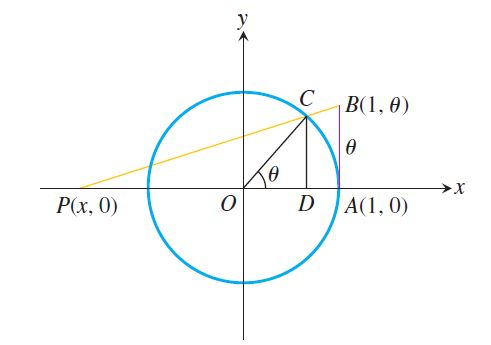
\includegraphics[scale=0.5]{img/20211211_01.JPG}\newline 
the circle has radius $OA$ equal to 1, and $AB$ is tangent to the circle at $A$. The arc $AC$ has radian measure $\theta$ and the segment $AB$ also has length $\theta$. The line through $B$ and $C$ crosses the x-axis at $P(x,0)$.
\begin{enumerate}[label=\textbf{\alph*.}]
    \item Show that the length of $PA$ is 
    \[1-x=\frac{\theta(1-\cos\theta)}{\theta-\sin\theta}\]
    \item Find $\lim_{\theta \to 0} (1-x)$.
    \item Show that $\lim _{\theta \to \infty} [(1-x)-(1-\cos\theta)]=0$.
\end{enumerate}
\subsection*{Solution.}
\begin{enumerate}[label=\textbf{\alph*.}]
    \item Let $Q$ be the projection of $C$ on segment $AB$.
    Clearly, $\Delta PAB\sim \Delta CQB$. So it can be seen that
    \[\frac{\overline{PA}}{\overline{AB}}=\frac{\overline{CQ}}{\overline{QB}}\]
    \[\Leftrightarrow \frac{1-x}{\theta}=\frac{1-\cos\theta }{\theta-\sin\theta}\]
    \[\Leftrightarrow 1-x=\frac{\theta(1-\cos\theta)}{\theta-\sin\theta}\text{     }\square\]
    \item 
    \[\lim_{\theta\to 0} (1-x)=\lim_{\theta\to 0} \frac{\theta(1-\cos\theta)}{\theta-\sin\theta}=\lim_{\theta\to 0} \frac{1-\cos\theta+\theta\sin\theta}{1-\cos\theta}=1+\lim_{\theta\to 0} \frac{\sin\theta+\theta\cos\theta}{\sin\theta}=2+\lim_{\theta\to 0} \frac{\theta}{\tan\theta}=3\]
    \item 
    \[\lim_{\theta\to\infty}[(1-x)-(1-\cos\theta)]=\lim_{\theta\to\infty}\frac{\theta(1-\cos\theta)-(\theta-\sin\theta)(1-\cos\theta)}{\theta-\sin\theta}=\lim_{\theta\to\infty} \frac{\sin\theta(1-\cos\theta)}{\theta-\sin\theta}\]
    Since $|\frac{\sin\theta}{\theta}|\leq \frac{1}{|\theta|}$, we have 
    \[\lim _{\theta\to\infty}\frac{\sin\theta}{\theta}=0,\]
    Moreover,
    \[0\leq\frac{\sin\theta(1-\cos\theta)}{\theta-\sin\theta}\leq \frac{2\sin\theta}{\theta-\sin\theta}\]
    so
    \[0\leq\lim_{\theta\to\infty} \frac{\sin\theta(1-\cos\theta)}{\theta-\sin\theta}\leq\lim_{\theta\to\infty} \frac{2\frac{\sin\theta}{\theta}}{1-\frac{\sin\theta}{\theta}}=\frac{0}{1-0}=0\]
    Thus
    \[\lim _{\theta \to \infty} [(1-x)-(1-\cos\theta)]=0 \text{     } \blacksquare\]
\end{enumerate}
\section*{Additional/Advanced Exercises.}
\subsection*{8.}
\textbf{An inequality} 
\begin{enumerate}[label=\textbf{\alph*.}]
    \item Show that $-1/2\leq x/(1+x^2)\leq 1/2$ for every value of $x$.
    \item Suppose that $f$ is a function whose derivative is $f'(x)=x/(1+x^2)$. Use the result in part (a) to show that \[|f(b)-f(a)|\leq \frac{1}{2}|b-a|\]
    for any $a$ and $b$.
\end{enumerate}
\subsection*{Solution.}
\begin{enumerate}[label=\textbf{\alph*.}]
    \item \[-1/2\leq x/(1+x^2)\leq 1/2\]
    \[\Leftrightarrow \left|\frac{x}{1+x^2}\right|\leq\frac{1}{2}\]
    \[\Leftrightarrow 2|x|\leq 1+x^2\]
    \[\Leftrightarrow (|x|-1)^2\geq 0\]
    The last statement holds as $\forall a\in\mathbf{R},a^2\geq 0$.  $\square$
    \item $f'$ is continuous over $\mathbf{R}$, hence Lagrange's mean value theorem can be used.\newline
    If $a=b$, then the inequality clearly holds.
    W.L.O.G., assume $a<b$.
    Then $\exists x_0\in (a,b)$ s.t. 
    \[f'(x_0)=\frac{f(b)-f(a)}{b-a}\]
    It is proved in part (a) that $\forall x\in \mathbf{R}, |f'(x)|=\left|\frac{x}{1+x^2}\right|\leq 1/2$, so
    \[\left|\frac{f(b)-f(a)}{b-a}\right|=|f'(x_0)|=\left|\frac{x_0}{1+x_0^2}\right|\leq \frac{1}{2}\]
    \[\Rightarrow |f(b)-f(a)|\leq \frac{1}{2}|b-a|\text{   }\blacksquare\]
\end{enumerate}
    
\subsection*{14.}
\textbf{Proving the second derivative test  } The Second Derivative Test for Local Maxima and Minima (Section 4.4) says:
\begin{enumerate} [label=\textbf{\alph*.}]
    \item $f$ has a local maximum value at $x=c$ if $f'(c)=0$ and $f''(c)<0$
    \item $f$ has a local minimum value at $x=c$ if $f'(c)=0$ and $f''(c)>0$
\end{enumerate}
To prove statement (a), let $\epsilon=(1/2)|f''(c)|$. Then use the fact that 
\[f''(c)=\lim_{h\to 0}\frac{f'(c+h)-f'(c)}{h}=\lim_{h\to 0} \frac{f'(c+h)}{h}\]
to conclude that for some $\delta>0$,\
\[0<|h|<\delta \Rightarrow \frac{f'(c+h)}{h}<f''(c)+\epsilon<0.\]
Thus, $f'(c+h)$ is positive for $-\delta<h<0$ and negative for $0<h<\delta$. Prove statement (b) in a similar way.
\subsection*{Solution.}
\[f''(c)=\lim_{h\to 0} \frac{f'(c+h)-f'(c)}{h}=\lim_{h\to 0} \frac{f'(c+h)}{h}\]
Hence, \[\forall \epsilon>0,\exists\delta>0,\forall h\in \mathring{U}(0,\delta),|\frac{f'(c+h)}{h}-f''(c)|<\epsilon\]
Let $\epsilon=\frac{1}{2}|f''(c)|$.
\[\Rightarrow -\frac{1}{2}|f''(c)|+f''(c)<\frac{f'(c+h)}{h}<\frac{1}{2}|f''(c)|+f''(c)\]
\begin{enumerate} [label=\textbf{\alph*.}]
    \item $f''(c)<0$. Then
    \[\frac{3}{2}f''(c)<\frac{f'(c+h)}{h}<\frac{1}{2}f''(c)<0\]
    For any $h$ in the right neighborhood of 0, $f'(c+h)<0$.\newline
    For any $h$ in the left neighborhood of 0, $f'(c+h)>0$. So $f(c)$ is a local maximum.
    \item $f''(c)>0$. Then
    \[0<\frac{1}{2}f''(c)<\frac{f'(c+h)}{h}<\frac{3}{2}f''(c)\]
    For any $h$ in the right neighborhood of 0, $f'(c+h)>0$.\newline
    For any $h$ in the left neighborhood of 0, $f'(c+h)<0$. So $f(c)$ is a local minimum.
\end{enumerate}
\subsection*{26.}
Let $f(x)$, $g(x)$ be two continuously differentiable  functions satisfying the relationships $f'(x)=g(x)$ and $f''(x)=-f(x)$. Let $h(x)=f^2(x)+g^2(x)$. If $h(0)=5$, find $h(10)$.
\subsection*{Solution.}
\[\forall x\in\mathbf{R}, g'(x)=f''(x)=-f(x)\]
\[h'(x)=2f(x)f'(x)+2g(x)g'(x)=2f(x)g(x)-2g(x)f(x)=0\]
Hence $h$ is a constant function, so $h(10)=h(0)=5$.
\end{document}